\documentclass[12pt, a4paper, oneside, fontset=windows]{ctexart}
\usepackage{amsmath, amsthm, amssymb, appendix, bm, graphicx, hyperref, mathrsfs,listings,xcolor}

\title{\textbf{大数据管理方法与应用第三次作业}}
\author{大数据001\\郅啸淇\\学号:2184114639}
\date{\today}
\linespread{1.5}
\lstset{
    basicstyle          =   \sffamily,          % 基本代码风格
    keywordstyle        =   \bfseries,          % 关键字风格
    commentstyle        =   \rmfamily\itshape,  % 注释的风格,斜体
    stringstyle         =   \ttfamily,  % 字符串风格
    flexiblecolumns,                % 别问为什么,加上这个
    numbers             =   left,   % 行号的位置在左边
    showspaces          =   false,  % 是否显示空格,显示了有点乱,所以不现实了
    numberstyle         =   \zihao{-5}\ttfamily,    % 行号的样式,小五号,tt等宽字体
    showstringspaces    =   false,
    captionpos          =   t,      % 这段代码的名字所呈现的位置,t指的是top上面
    frame               =   lrtb,   % 显示边框
}

\lstdefinestyle{Python}{
    language        =   Python, % 语言选Python
    basicstyle      =   \zihao{-5}\ttfamily,
    numberstyle     =   \zihao{-5}\ttfamily,
    keywordstyle    =   \color{blue},
    keywordstyle    =   [2] \color{teal},
    stringstyle     =   \color{magenta},
    commentstyle    =   \color{red}\ttfamily,
    breaklines      =   true,   % 自动换行,建议不要写太长的行
    columns         =   fixed,  % 如果不加这一句,字间距就不固定,很丑,必须加
    basewidth       =   0.5em,
}
\lstdefinestyle{Matlab}{
    language        =   Matlab, % 语言选Matlab
    basicstyle      =   \zihao{-5}\ttfamily,
    numberstyle     =   \zihao{-5}\ttfamily,
    keywordstyle    =   \color{blue},
    keywordstyle    =   [2] \color{teal},
    stringstyle     =   \color{magenta},
    commentstyle    =   \color{red}\ttfamily,
    breaklines      =   true,   % 自动换行,建议不要写太长的行
    columns         =   fixed,  % 如果不加这一句,字间距就不固定,很丑,必须加
    basewidth       =   0.5em,
}
\newtheorem{theorem}{定理}[section]
\newtheorem{definition}[theorem]{定义}
\newtheorem{lemma}[theorem]{引理}
\newtheorem{corollary}[theorem]{推论}
\newtheorem{example}[theorem]{例}
\newtheorem{proposition}[theorem]{命题}
\begin{document}
\maketitle
\newpage
%\tableofcontents
\newpage
\section{抛硬币的后验分布}
\subsection{分布与图像}
由课堂证明已知,抛硬币的后验分布为$P(\theta |x) = Beta(\theta|a+x,b+n-x)$,将不同参数的各组数据分布情况绘图如图1所示。
\begin{figure}[h]
    \centering
    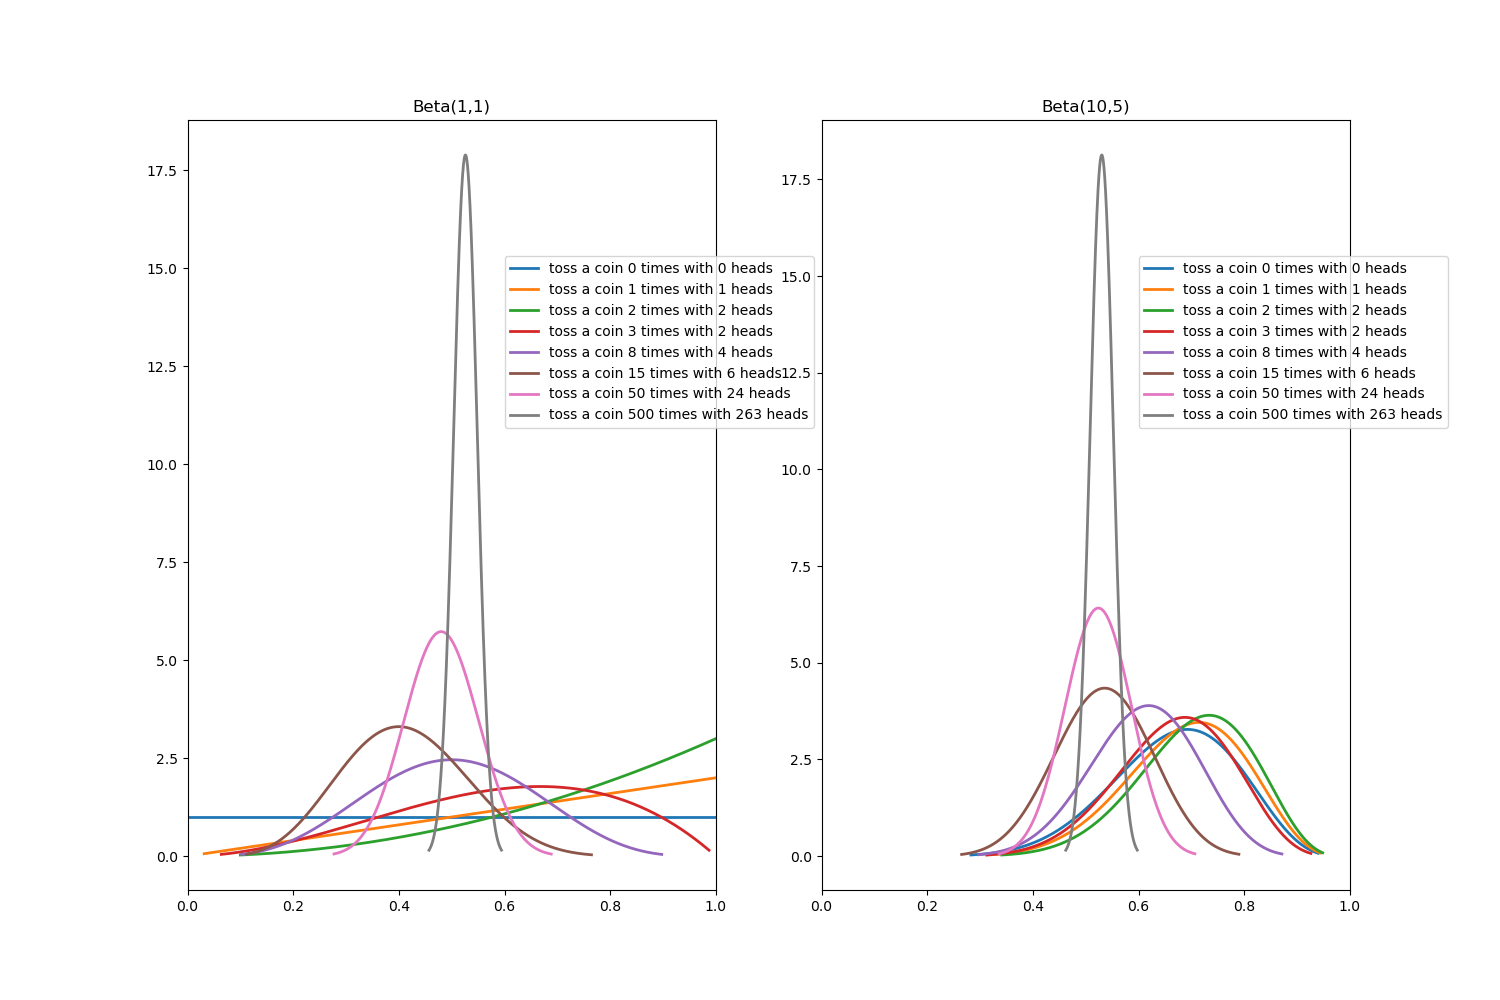
\includegraphics[scale = 0.4]{tossCoin.png}
    \caption{分布情况}
\end{figure}
\newpage
\subsection{完整代码}
\lstinputlisting[style=Python]{Beta.py}
\section{共轭先验的证明}
\subsection{证明多项分布的共轭先验是狄利克雷分布}
似然函数为多项分布,其中$\theta_i$代表第i类出现的概率,$n_i$代表第i类出现的次数。

多项分布的先验分布$P(x|\theta) = \frac{n!}{n_1!n_2!n_3!n_4!...n_k!} \prod_{i = 1}^{k} \theta_{i}^{n^{i}}$,其中$\sum_{i = 1}^{k} \theta_i  =1$

使用Gamma函数对阶乘进行近似,有$\Gamma(x+1) = x!$,则$P(x|\theta) = \frac{\Gamma(n+1)}{\sum_{i = 1}^{k} \Gamma(n_i + 1)} \prod_{i = 1}^{k} \theta_i^{n_i}$

假设概率$\theta = (\theta_1,\theta_2,...,\theta_k)$的先验分布为参数是$\alpha = (\alpha_1,\alpha_2,\alpha_3,...,\alpha_k)$的狄利克雷分布$Dir(\alpha)$

有$P(\theta) = \frac{\Gamma(\sum_{i = 1}^{k} \alpha_i)}{\prod_{i=1}^{k} \Gamma(\alpha_i)} \prod_{i = 1}^{k} \theta_i^{\alpha_{i} - 1}$

计算
\begin{align*}
P(x)& = \int P(x|\theta)P(\theta) d\theta\\
    & = \int_0^1 \frac{\Gamma(n+1)}{\prod_{i=1}^{k} \Gamma(n_i + 1)}\prod_{i=1}^{k} \theta_i^{n_i}  \frac{\Gamma(\sum_{i=1}^{k}\alpha_i)}{\prod_{i=1}^{k}\Gamma(\alpha_i)} \prod_{i=1}^{k}\theta_{i}^{\alpha_i - 1} d\theta\\
    & = \frac{\Gamma(n+1)\Gamma(\sum_{i=1}^{k}\alpha_i)}{\prod_{i=1}^{k} \Gamma(n_i + 1)\Gamma(\alpha_i)} \frac{\prod_{i=1}^{k} \Gamma(n_i + \alpha_i)}{\Gamma(\sum_{i=1}^{k} n_i + \alpha_i)} \int_0^1 \frac{\Gamma(\sum_{i=1}^{k} n_i + \alpha_i)}{\prod_{i=1}^{k} \Gamma(n_i + \alpha_i)} \prod_{i=1}^{k} \theta_i^{\alpha_i + n_i -1}d\theta\\
    & = \frac{\Gamma(n+1)\Gamma(\sum_{i=1}^{k}\alpha_i)}{\prod_{i=1}^{k} \Gamma(n_i + 1)\Gamma(\alpha_i)} \frac{\prod_{i=1}^{k} \Gamma(n_i + \alpha_i)}{\Gamma(\sum_{i=1}^{k} n_i + \alpha_i)} \int_0^1 Dir(n + \alpha)d\theta\\
    & = \frac{\Gamma(n+1)\Gamma(\sum_{i=1}^{k}\alpha_i)}{\prod_{i=1}^{k} \Gamma(n_i + 1)\Gamma(\alpha_i)} \frac{\prod_{i=1}^{k} \Gamma(n_i + \alpha_i)}{\Gamma(\sum_{i=1}^{k} n_i + \alpha_i)}
\end{align*}

然后计算$\theta$的后验分布
\begin{align*}
    P(\theta \mid x) &= \frac{P(x \mid \theta)P(\theta)}{P(x)}\\
    &=\frac{\frac{\Gamma(n+1)}{\prod_{i=1}^k \Gamma(n_i+1)}\prod_{i=1}^k \theta_i^{n_i}\frac{\Gamma(\sum_{i=1}^k \alpha_i)}{\prod_{i=1}^{k} \Gamma(\alpha_{i})} \prod_{i=1}^{k} \theta_{i}^{\alpha_{i}-1}}{\frac{\Gamma(n+1)\Gamma(\sum_{i=1}^k \alpha_i)}{\Gamma(\sum_{i=1}^k n_i+\alpha_{i})}\prod_{i=1}^{k} \frac{\Gamma(n_i+\alpha_{i})}{\Gamma(n_i+1)\Gamma(\alpha_i)}}\\
    &=\frac{\Gamma(\sum_{i=1}^k n_i+\alpha_i)}{\prod_{i=1}^{k}\Gamma(n_i+\alpha_{i})}\prod_{i=1}^{k} \theta_i^{n_i+\alpha_{i}-1}\\
    &=Dir(n+\alpha)
\end{align*}
得到$\theta$先验分布和后验分布均为狄利克雷分布,且似然函数为多项分布,故多项分布的共轭先验为狄利克雷分布
\subsection{证明泊松分布的共轭先验为伽马分布}
似然函数是指数分布,n代表事件发生次数,$\lambda$代表单位时间内随机事件的平均发生次数

则有先验分布$P(x = n \mid \lambda) = \lambda e^{-\lambda x}$

假设$\lambda$服从参数为$(a,b)$的伽马分布
$P(\lambda) = \frac{\lambda^{a-1}e^{-b \lambda}b^a}{\Gamma(a)}$

计算$P(x)$
\begin{align*}
    P(x) &= \int P(x \mid \lambda) P(\lambda) d\lambda\\
    &=\int_0^1 \lambda e^{-\lambda x}\frac{\lambda^{a-1}e^{-b \lambda} b^a}{\Gamma(a)} d\lambda\\
    &=\frac{b^a}{\Gamma(a)}\frac{\Gamma(a+1)}{(b+1)^{a+1}} \int_0^1 \lambda^{a} e^{-(b+1)\lambda} \frac{(b+1)^{a+1}}{\Gamma(a+1)} d\lambda\\
    &= \frac{b^a}{\Gamma(a)}\frac{\Gamma(a+1)}{(b+1)^{a+1}} \int_0^1 Ga(a+1,b+1) d\lambda\\
    &= \frac{b^a}{\Gamma(a)}\frac{\Gamma(a+1)}{(b+1)^{a+1}}
\end{align*}

得到$\lambda$的后验分布
\begin{align*}
    P(\lambda \mid x) &= \frac{P(x \mid \lambda)P(\lambda)}{P(x)}\\
    &=\frac{\lambda e^{-\lambda x}\frac{\lambda^{a-1}e^{-b \lambda} b^a}{\Gamma(a)}}{\frac{b^a}{\Gamma(a)}\frac{\Gamma(a+1)}{(b+1)^{a+1}}}\\
    &=\frac{(b+1)^{a+1}}{\Gamma(a+1)}\lambda^{a} e^{-(b+1)\lambda}\\
    &=Ga(a+1,b+1)
\end{align*}

$\lambda$的先验和后验分布都是伽马分布,似然函数是泊松分布,所以泊松分布的共轭先验是伽马分布
\subsection{证明方差已知的正态分布的共轭先验是正态分布}
似然函数是方差已知的正态分布,有$P(x \mid \mu)=\frac{1}{\sigma \sqrt{2 \pi}} e^{-\frac{1}{2}\left(\frac{x-\mu}{\sigma}\right)^{2}}$

假设$\mu$服从参数为$(a,b^2)$的正态分布$\mu\sim N(a,b^2)$,则有

$P(\mu)=\frac{1}{b \sqrt{2 \pi}} e^{-\frac{1}{2}\left(\frac{\mu-a}{b}\right)^{2}}$

计算$P(x)$
\begin{align*}
    P(x) &= \int P(x \mid \mu) P(\mu) d\mu\\
    &=\int_{-\infty}^{\infty} \frac{1}{\sigma \sqrt{2 \pi}} e^{-\frac{1}{2}\left(\frac{x-\mu}{\sigma}\right)^{2}}\frac{1}{b \sqrt{2 \pi}} e^{-\frac{1}{2}\left(\frac{\mu-a}{b}\right)^{2}} d\mu\\
    &=\frac{1}{2 \sigma b \pi}\int_{-\infty}^{\infty} e^{-\frac{1}{2}\frac{(x-\mu)^2b^2+(\mu-a)^2\sigma^2}{\sigma^2 b^2}} d\mu\\
    &=\frac{1}{2 \sigma b \pi}\int_{-\infty}^{\infty}exp\left(-\frac{1}{2}\left(\frac{\left(\mu-\frac{xb^2+a\sigma^2}{\sigma^2+b^2}\right)^2}{\frac{\sigma^2b^2}{\sigma^2+b^2}}+\frac{(x-a)^2}{\sigma^2+b^2}\right)\right)d\mu\\
    &=\frac{e^{-\frac{1}{2}\frac{(x-a)^2}{\sigma^2+b^2}}}{2 \sigma b \pi}\frac{\sigma b}{\sqrt{\sigma^2+b^2}}\sqrt{2 \pi}\int_{-\infty}^{\infty}\frac{1}{\frac{\sigma b}{\sqrt{\sigma^2+b^2}}\sqrt{2 \pi}}exp\left(-\frac{1}{2}\left(\frac{\left(\mu-\frac{xb^2+a\sigma^2}{\sigma^2+b^2}\right)^2}{\frac{\sigma^2b^2}{\sigma^2+b^2}}\right)\right)d\mu\\
    &=\frac{1}{\sqrt{\sigma^2+b^2}\sqrt{2 \pi}}e^{-\frac{1}{2}\frac{(x-a)^2}{\sigma^2+b^2}}\int_{-\infty}^{\infty} \mu\sim N\left(\frac{xb^2+a\sigma^2}{\sigma^2+b^2},\frac{\sigma b}{\sqrt{\sigma^2+b^2}}\right)d\mu\\
    &=\frac{1}{\sqrt{\sigma^2+b^2}\sqrt{2 \pi}}e^{-\frac{1}{2}\frac{(x-a)^2}{\sigma^2+b^2}}
\end{align*}

计算$\mu$的后验分布
\begin{align*}
    P(\mu \mid x) &= \frac{P(x \mid \mu)P(\mu)}{P(x)}\\
    &=\frac{\frac{1}{\sigma \sqrt{2 \pi}} e^{-\frac{1}{2}\left(\frac{x-\mu}{\sigma}\right)^{2}}\frac{1}{b \sqrt{2 \pi}} e^{-\frac{1}{2}\left(\frac{\mu-a}{b}\right)^{2}}}{\frac{1}{\sqrt{\sigma^2+b^2}\sqrt{2 \pi}}e^{-\frac{1}{2}\frac{(x-a)^2}{\sigma^2+b^2}}}\\
    &=\frac{\sqrt{\sigma^2+b^2}}{\sigma b\sqrt{2 \pi}}e^{-\frac{1}{2}\left(\left(\frac{x-\mu}{\sigma}\right)^{2}+\left(\frac{\mu-a}{b}\right)^{2}-\frac{(x-a)^2}{\sigma^2+b^2}\right)}\\
    &=\frac{1}{\frac{\sigma b}{\sqrt{\sigma^2+b^2}}\sqrt{2 \pi}}e^{-\frac{1}{2}\frac{\left(\mu-\frac{xb^2+a\sigma^2}{\sigma^2+b^2}\right)^2}{\frac{\sigma^2b^2}{\sigma^2+b^2}}}\\
    &=N\left(\frac{xb^2+a\sigma^2}{\sigma^2+b^2},\frac{\sigma b}{\sqrt{\sigma^2+b^2}}\right)
\end{align*}

$\lambda$的先验和后验分布都是正态分布,似然函数是正态分布分布,所以方差已知的正态分布的共轭先验是正态分布

\subsection{证明均值已知的正态分布的共轭先验是逆伽马分布}
似然函数是均值已知的正态分布,则有$P(x\mid \sigma^2)=\frac{1}{\sigma \sqrt{2 \pi}} e^{-\frac{1}{2}\left(\frac{x-\mu}{\sigma}\right)^{2}}$

假设参数$\sigma^2$服从参数为$(a,b)$的逆伽马分布$\sigma^2 \sim IGa(a,b)$

$p(\sigma^2)=\frac{b^a}{\Gamma(a)}\left(\frac{1}{\sigma^2}\right)^{a+1} e^{-\frac{b}{\sigma^2}}$

计算$P(x)$
\begin{align*}
    P(x) &= \int P(x\mid \sigma^2) P(\sigma^2) d\sigma^2\\
    &=\int_{0}^{\infty}\frac{1}{\sigma \sqrt{2 \pi}} e^{-\frac{1}{2}\left(\frac{x-\mu}{\sigma}\right)^{2}} \frac{b^a}{\Gamma(a)}\left(\frac{1}{\sigma^2}\right)^{a+1} e^{-\frac{b}{\sigma^2}} d\sigma^2\\
    &=\frac{1}{\sqrt{2 \pi}}\frac{b^a}{\Gamma(a)}\int_{0}^{\infty}\left(\frac{1}{\sigma^2}\right)^{a+\frac{3}{2}} e^{-\frac{b}{\sigma^2}-\frac{1}{2}\left(\frac{x-\mu}{\sigma}\right)^{2}} d\sigma^2\\
    &= \frac{1}{\sqrt{2 \pi}}\frac{b^a}{\Gamma(a)}\frac{\Gamma(a+\frac{1}{2})}{\left(b+\frac{1}{2}\left(x-\mu\right)^{2}\right)^{a+\frac{1}{2}}}\int_{0}^{\infty}\frac{\left(b+\frac{1}{2}\left(x-\mu\right)^{2}\right)^{a+\frac{1}{2}}}{\Gamma(a+\frac{1}{2})}\left(\frac{1}{\sigma^2}\right)^{a+1+\frac{1}{2}} e^{-\frac{b+\frac{1}{2}\left(x-\mu\right)^{2}}{\sigma^2}} d\sigma^2\\
    &=\frac{1}{\sqrt{2 \pi}}\frac{b^a}{\Gamma(a)}\frac{\Gamma(a+\frac{1}{2})}{\left(b+\frac{1}{2}\left(x-\mu\right)^{2}\right)^{a+\frac{1}{2}}}\int_{0}^{\infty}\sigma^2 \sim IGa\left(a+\frac{1}{2},b+\frac{1}{2}\left(x-\mu\right)^{2}\right) d\sigma^2\\
    &=\frac{1}{\sqrt{2 \pi}}\frac{\Gamma(a+\frac{1}{2})}{\Gamma(a)}\frac{b^a}{\left(b+\frac{1}{2}\left(x-\mu\right)^{2}\right)^{a+\frac{1}{2}}}
\end{align*}
计算后验分布
\begin{align*}
    P(\sigma^2\mid x) &= \frac{P(x\mid \sigma^2)P(\sigma^2)}{P(x)}\\
    &=\frac{\frac{1}{\sigma \sqrt{2 \pi}} e^{-\frac{1}{2}\left(\frac{x-\mu}{\sigma}\right)^{2}} \frac{b^a}{\Gamma(a)}\left(\frac{1}{\sigma^2}\right)^{a+1} e^{-\frac{b}{\sigma^2}}}{\frac{1}{\sqrt{2 \pi}}\frac{\Gamma(a+\frac{1}{2})}{\Gamma(a)}\frac{b^a}{\left(b+\frac{1}{2}\left(x-\mu\right)^{2}\right)^{a+\frac{1}{2}}}}\\
    &=\frac{\left(b+\frac{1}{2}\left(x-\mu\right)^{2}\right)^{a+\frac{1}{2}}}{\Gamma(a+\frac{1}{2})}\left(\frac{1}{\sigma^2}\right)^{a+1+\frac{1}{2}}e^{-\frac{b+\frac{1}{2}\left(x-\mu\right)^{2}}{\sigma^2}}\\
    &=IGa\left(a+\frac{1}{2},b+\frac{1}{2}\left(x-\mu\right)^{2}\right)
\end{align*}

$\mu$的先验和后验分布都是逆伽马函数,似然函数是正态分布分布,所以均值已知的正态分布的共轭先验是逆伽马分布
\end{document} 